\documentclass[11pt]{beamer}
\usetheme{Frankfurt}
\usepackage[utf8]{inputenc}
\usepackage[french]{babel}
\usepackage[T1]{fontenc}
\usepackage{amsmath}
\usepackage{amsfonts}
\usepackage{amssymb}
\usepackage{graphicx}
\usepackage{hyperref}
\usepackage{eurosym}
\usepackage{smartdiagram}
%\usepackage{smartdiagram}
%\usecolortheme{crane}

%\definecolor{fondtitre}{rgb}{0.20,0.43,0.09}  % vert fonce
\definecolor{coultitre}{rgb}{1,0.6,0.1}  % orange "logement"
\setbeamercolor{structure}{fg=coultitre, bg=coultitre!40}

\date{13 juin 2018}
\author{CGDD / SDES}
\title{Un maillage pour l'analyse territoriale de l'habitat \\ Présentation JMS}

\titlegraphic{
\includegraphics[width=3cm]{Logos/A4_Picto_Logement-Construction}\hspace*{4.75cm}~  
\includegraphics[width=1cm]{Logos/MTSE_MCT_RVB.png}
}

%\setbeamercovered{transparent} 
%\setbeamertemplate{navigation symbols}{} 
%\logo{} 
%\institute{} 
%\date{} 
%\subject{} 

\begin{document}

\begin{frame}
\titlepage
\end{frame}

\begin{frame}{Plan}
\begin{enumerate}

\item Motifs et Objectifs

\item Méthode de travail

\item Choix des indicateurs constitutifs

\item Choix des paramètres de la méthode de \emph{régionalisation}

\item Résultats 

\vfill
\end{enumerate}
\end{frame}

\section{Motifs et objectifs}

\begin{frame}{Constat}

Entre les zones d'emploi et les bassins de vie, manque d'une maille d'analyse du logement.
\vspace{.3cm}

\begin{itemize}
\item Demande croissante d'information localisée
\item La maille communale souvent choisie par défaut pour le logement
\end{itemize}
\vspace{.3cm}
$\Rightarrow$ exemple du projet de territorialisation des besoins en logement de la DHUP
\end{frame}

\begin{frame}{Objectifs}
\begin{enumerate}
\item Réaliser une partition du territoire
\item Approximer la notion de marché local du logement
\item Prendre en compte l'ensemble des dimensions de ce marché (offre - \emph{parc, qualité} -, et demande -\emph{démographie, solvabilité} -)
\item Faire en sorte que le zonage soit mobilisé aux niveaux national et local
\end{enumerate}
\end{frame}

\section{Méthode de travail}

\begin{frame}{Deux comités}

Deux comités ont été constitués par appel à manifestation d'intérêt :
\begin{itemize}
\item Comité de pilotage :\
\begin{enumerate}
\item DREAL : services habitats et / ou connaissance
\item FNAU
\item Cerema
\item Insee (DDAR, DMSCI, Division Logement)
\item CGET
\item DHUP
\item \'Ecole d'urbanisme de Paris
\end{enumerate}
\item Comité technique : davantage de régionaux, notamment statisticien(ne)s. PSAR Analyse territoriale et synthèse locale Insee.
\end{itemize}
\end{frame}

\begin{frame}{Méthode de travail : deux sous-processus}
\begin{center}
\begin{tabular}{c c c}
Première étape & \hspace{2cm} & Seconde étape \\
\smartdiagram[flow diagram]{
  Choix analyse des indicateurs,
  Analyse des indicateurs,
  Classification non contrainte
  }
&  \hspace{2cm} &
 \smartdiagram[flow diagram]{ 
  Méthode de régionalisation,
  Réalisation du zonage,
  Concertation et recettage
  }
\end{tabular}
\end{center}
\end{frame}


\begin{frame}{Les orientations prises}
Les grandes lignes directrices issues des comités et des travaux de l'équipe projet : 
\begin{enumerate}
\item Privilégier une maille communale comme maille initiale 
\item Centrer les variables constitutives du maillage sur des indicateurs relevant spécifiquement du logement, en évitant d'introduire des variables trop générales.
\item Livrer un \emph{outil}
\item Limitation du nombre d'indicateurs à mobiliser
\item Choix de l'algorithme SKATER pour la régionalisation 
\end{enumerate}
\end{frame}

\section{ Indicateurs constitutifs}

\begin{frame}{Les indicateurs}

\begin{enumerate}
\small{
\item Nombre de personnes par ménage
\item Part de résidences secondaires
\item Part de logements vacants
\item Indice de jeunesse du parc (part post 75 / part ante 49)
\item Le prix des logements anciens au $m^2$  rapporté au revenu médian communal
\item La part de logements sociaux
\item La durée d'occupation des logements (permet de prendre en compte les statuts d'occupation)
\item La part de logements sur-occupés
\item Taux de transactions dans l'ancien
}
\end{enumerate}
\end{frame}

\begin{frame}{Classification des communes}
\begin{center}
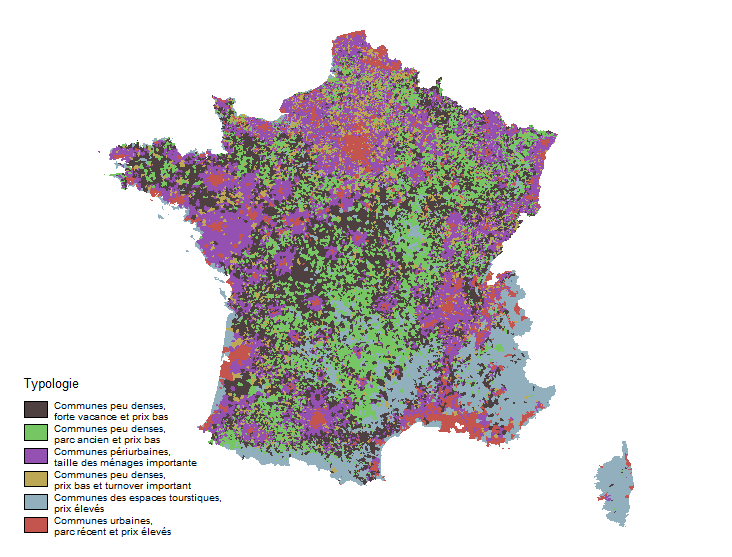
\includegraphics[scale=.5]{img/Typo_com}
\end{center}
\end{frame}


\section{La régionalisation}

\begin{frame}{Algorithme de régionalisation}
Les grandes étapes de l'algorithme SKATER (Spatial Kluster Analysis by Tree Edge Removal) :
\begin{itemize}
\item Construction de la matrice de contiguïté $\rightarrow$ obtention d'un graphe
\item Pondération du graphe à partir des distances calculées sur les indicateurs
\item Construction de l'arbre portant minimal en retenant le lien le plus "fort" pour chaque n\oe ud du graphe 
\item Suppression itérative des branches de l'arbre minimisant la différence entre variance totale et somme des variances des sous-arbres résultant de la coupure
\end{itemize}
\end{frame}

\begin{frame}{Construction de l'arbre portant minimal}
\begin{center}
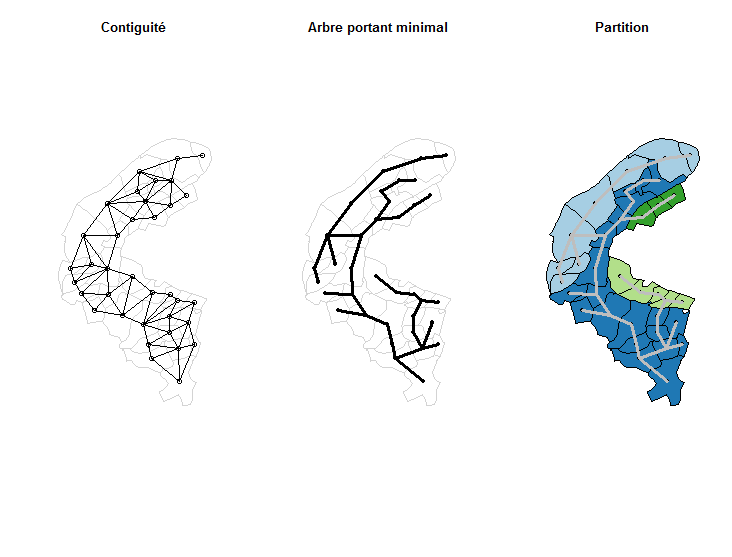
\includegraphics[scale=.55]{img/SKATER}
\end{center}
\end{frame}

\begin{frame}{Les simulations}

L'algorithme fonctionne avec deux paramètres :
\begin{enumerate}
\item Le nombre total de zones voulues (on utilise le nombre moyen de commune par zone pour le déterminer)
\item Une taille minimale des zones (nombre de commune, population...)
\end{enumerate}
\vspace{.2cm}
\underline{Difficulté :} l'algorithme est trop coûteux ( > $o(n^2)$) pour être exécuté sur l'ensemble des communes, on procède donc région par région puis on "lisse" les frontières régionales pour les éliminer.

\vspace{.2cm}

16 simulations ont été menées en faisant varier le nombre de communes par zone entre 20 et 80 et une taille limite entre 40000 et 50000 habitants.
\end{frame}

\begin{frame}{Lissage des limites régionales}
On identifie les communes des mailles situées le long des frontières régionales et on les répartit dans des macro-zones :
\begin{center}
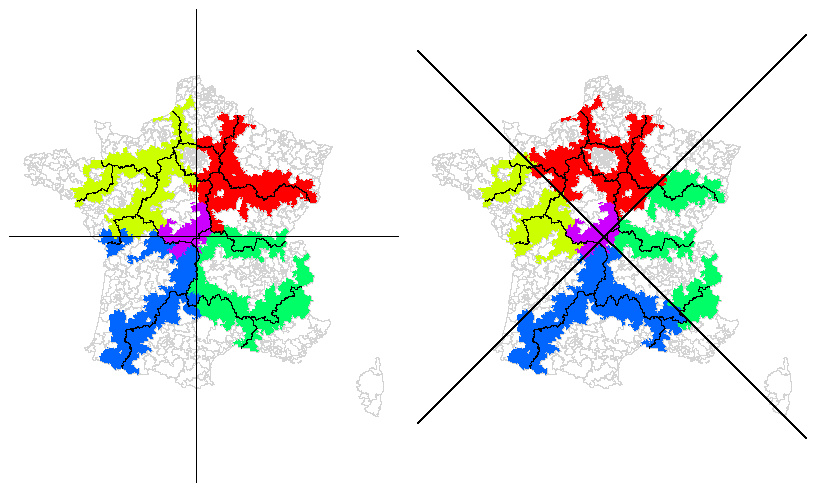
\includegraphics[scale=.5]{img/Methodo_decoupage}
\end{center}
\end{frame}


\begin{frame}{Quelques enseignements des simulations}
\begin{itemize}
\item Le temps de calcul croît exponentiellement avec le nombre de communes (3 heures pour la région Grand-Est vs. quelques minutes pour l'Île de France) ;
\item Le c\oe ur des aires urbaines constitue une zone à part entière ;
\item La limite de taille est la contrainte la plus forte $\Rightarrow$ augmenter le nombre de zones conduit à découper plus finement les espaces urbains
\item L'ensemble des simulation donne un bon lissage des indicateurs au niveau national (cartes lisibles)
\end{itemize}
\end{frame}

\section{Résultats}

\begin{frame}{Le maillage retenu}
Après concertation, on retient de scénario 40 communes par maille et 40000 habitants minimum, soient 777 mailles.
\begin{center}
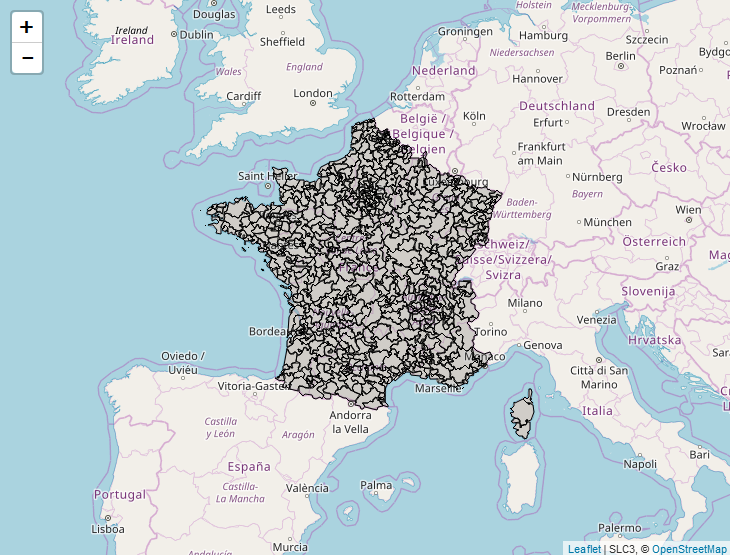
\includegraphics[scale=.5]{img/Maille}
\end{center}
\end{frame}

\begin{frame}{Les disparités apparaissent nettement}
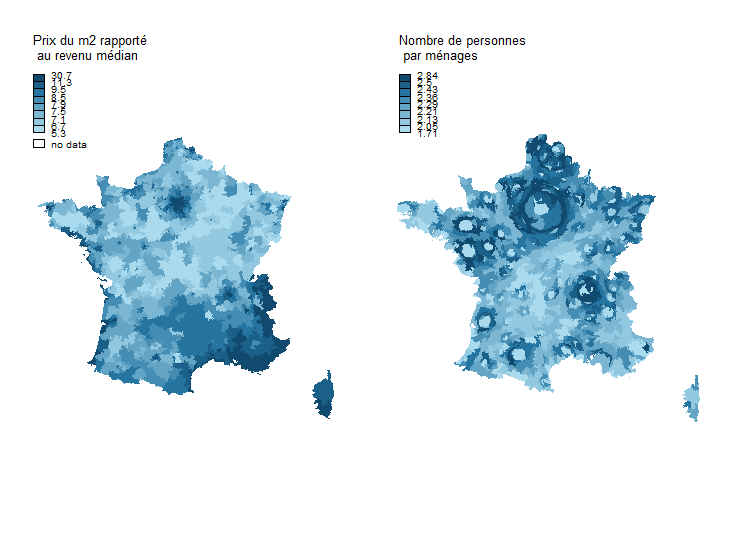
\includegraphics[scale=.6]{img/Discrim_mailles}
\end{frame}

\begin{frame}{L'habitat en exergue}

Le maillage obtenu permet de mettre en avant les disparités propres au logement

\begin{center}
\textbf{Principales disparités territoriales} \\
\vspace{.3cm}

\begin{tabular}{p{4cm} | p{4cm}}
\hline
Maille Communale & Maille logement \\
\hline
Degré d'urbanité & Degré de tension \\
Degré de tension & Taille des ménages \\
Zones touristiques & Zones touristiques \\
\hline

\end{tabular}
\end{center}
\end{frame}

\begin{frame}{Une typologie propre au logement}

La classification faite sur les zones met en lumière 6 types de zones, caractérisées par le logement :
\vspace{.2cm}
\begin{enumerate}
\item Mailles détendues à dominante rurale
\item Mailles peu tendues des couronnes périurbaines
\item Mailles assez tendues des pôles urbains de province
\item Mailles tendues des couronnes des aires urbaines attractives
\item Mailles tendues des espaces touristiques
\item Mailles à difficultés prononcées d'accès au logement
\end{enumerate}
\end{frame}


\begin{frame}{Une typologie propre au logement}
\begin{center}
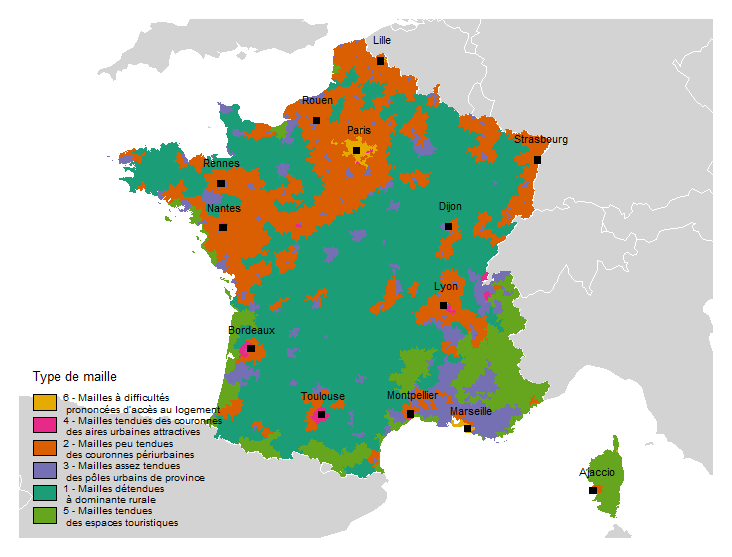
\includegraphics[scale=.55]{img/Typo_mailles}
\end{center}
\end{frame}

\begin{frame}{Homogénéité des mailles}
Davantage d'hétérogénéité dans les mailles peu tendues
\begin{center}
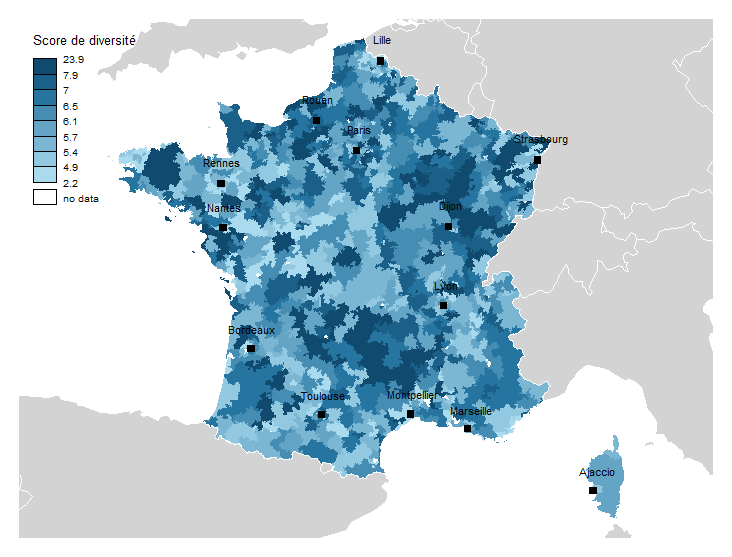
\includegraphics[scale=.5]{img/Diversite}
\end{center}
\end{frame}

\begin{frame}{Dynamiques de ces espaces}
Les spécificités des territoires se renforcent au cours du temps 
\begin{center}
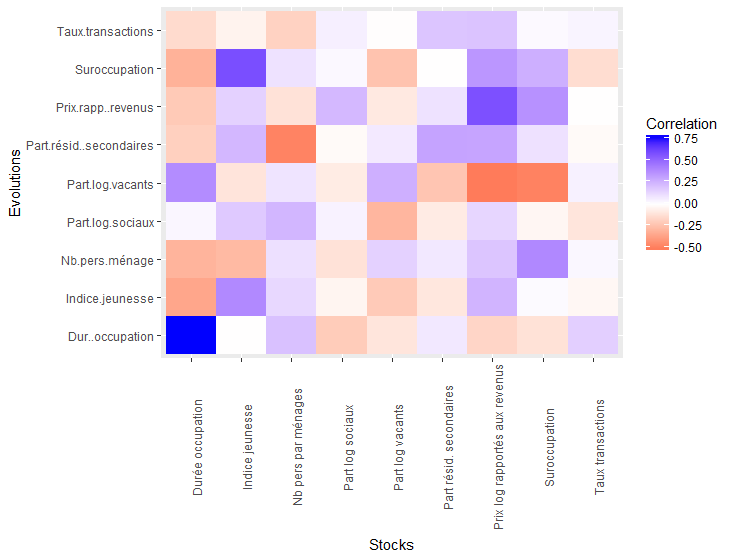
\includegraphics[scale=.5]{img/Dynam}
\end{center}
\end{frame}

\begin{frame}{Utilisation avec d'autres indicateurs}
\begin{center}
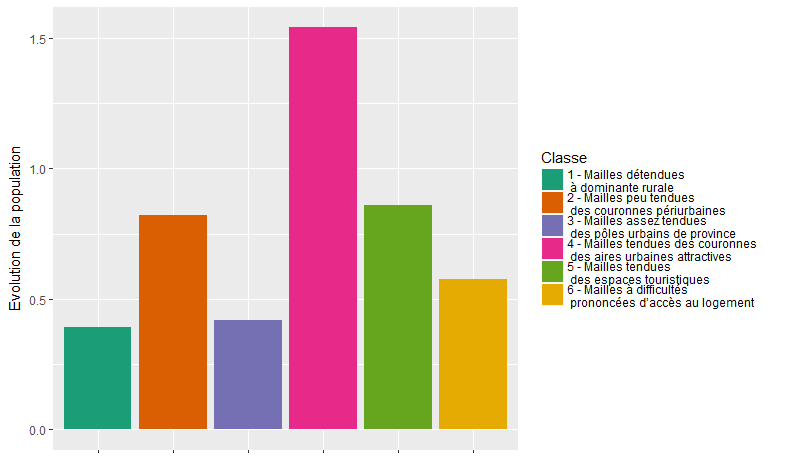
\includegraphics[scale=.55]{img/Evol_pop}
\end{center}
\end{frame}


\begin{frame}{Conclusion}

Le maillage habitat permet de saisir les disparités territoriales sur le domaine du logement et permet d'en apprécier la cohésion et les dynamiques. \
Ce projet propose plusieurs livrables :
\begin{itemize}
\item Le maillage sélectionné par les comités et la typologie finale
\item Une base de données communale avec les indicateurs constitutifs du zonage
\item L'ensemble des simulations qui ont été réalisées à des fins d'études spécifiques, avec les indicateurs constitutifs agrégés
\item Les codes sources des programmes de constitution des maillages
\item Une publication présentant les résultats ainsi qu'un manuel d'utilisation de l'ensemble des livrables
\end{itemize}
\end{frame}

\end{document}